\documentclass[12pt, letterpaper]{article}
\usepackage[hyphens]{url}
\setlength{\topmargin}{-1.75cm} \setlength{\textheight}{22.5cm}
\setlength{\oddsidemargin}{0.25cm}
\setlength{\evensidemargin}{0.25cm} \setlength{\textwidth}{16.2cm}
\renewcommand{\figurename}{Figure}
\usepackage{amssymb}
\usepackage{graphicx}
\usepackage{amsmath}
\usepackage{xcolor}
\usepackage[normalem]{ulem}
\usepackage{fontenc}
\usepackage{footnote}
\usepackage[breaklinks]{hyperref}
\usepackage{palatino, multicol, listings} % for multiple columns
\lstset{mathescape=true, basicstyle=\ttfamily,}

%\usepackage{pictex}
%% in the .pictex output of xfig, there is command \colo
%% however the old version of pictex may not define this
%% so we define color here as empty
%\def \color#1]#2{}

\begin{document}

\newcommand{\hide}[1]{}
\newcommand{\exercise}[1]{}
\newcommand{\future}[1]{}
\newcommand{\otherquestions}[1]{}
\newcommand{\set}[1]{\{#1\}}
\newcommand{\pg}[1]{{\tt #1}}
\newtheorem{definition}{Definition}
\newcommand{\emptyclause}{\Box}
\def\st{\bigskip\noindent}
\newcommand{\lplus}
{
   \stackrel{+}{\gets}
}

\newcommand{\fe}[1] {
  \begin{frame}
    #1
  \end{frame}}

\newcommand{\eoa}{ {\bf End} of algorithm}

\newcommand{\ft}[1] {\frametitle{#1}}

\newcommand{\ie}[1] {
  \begin{itemize}
    #1
  \end{itemize}
}

\newcommand{\ee}[1] {
  \begin{enumerate}
    #1
  \end{enumerate}\label{marker}
}
\newcommand{\blk}[2] {
  \begin{block}{#1}
    #2
  \end{block}
}

\newtheorem{collorary}{Corollary}
\newtheorem{proposition}{Proposition}
\newtheorem{invariant}{Invariant}
\newtheorem{property}{Property}
\newtheorem{claim}{Claim}
\newtheorem{example}{Example}


\title{P-log System manual}
\date{\today}
\maketitle
\tableofcontents
\pagebreak


\section{System installation}

For the latest instructions on system installation, please refer to \url{https://github.com/iensen/plog2.0/wiki/Installation-Instructions}.
\section{System usage}\label{sysusage}

\medskip\noindent
The system accepts ASCII files as inputs.
The file can be of any extension (we recommend .plog).

\medskip\noindent
A file acceptable by the system should consist of:
\begin{enumerate}
\item A P-log program, consisting of three sections:
\begin{itemize}
\item sorts definitions,
\item attribute declarations, and
\item program rules
\end{itemize}
\item A query.
\end{enumerate}

\st
For example, consider the following program, where sort definitions start with keywords \texttt{sorts}, attribute declarations start with keyword \texttt{attributes}, program rules start with keyword \texttt{statements}, and query starts with symbol \texttt{?}:
\begin{verbatim}
sorts

#dice={d1,d2}.
#score={1,2,3,4,5,6}.
#person={mike,john}.
#bool = {true,false}.


attributes

roll:#dice->#score.
owns:#dice,#person->#bool.

statements

owns(d1,mike).
owns(d2,john).

random(roll(D)).

%probability information

pr(roll(D)=6|owns(D,mike))=1/4.

? roll(d1)=1.
\end{verbatim}


The program, originally introduced in \cite{gelfond2014knowledge}, describes a scenario with two dice being rolled, belonging to Mike and John respectively.
Mike's die is more likely to produce \textit{6} as an outcome, as defined by the pr-atom
$$pr(roll(D)=6~|~owns(D,mike))=1/4.$$
By the so called \textit{principle of indifference} used by P-log, the probabilities of the remaining outcomes equal to (1 - 1/4)/5 = 3/20.
Thus, the answer to the query $roll(d1)=1$ is 3/20. Note that all outcomes of John's die are equally likely, so the answer to the query $roll(d2)=1$ is equal to 1/6.


\st
To compute the query probability using the system, we need to store it in a file and run the command:
$$plog2~[path\_to\_file]$$
where $plog2$ is the name of the p-log executable. For example, assuming the file is stored in $plogapp/tests/paper/dice1.plog$ in our system, we get the following output:

\begin{figure}[ht]
\centering
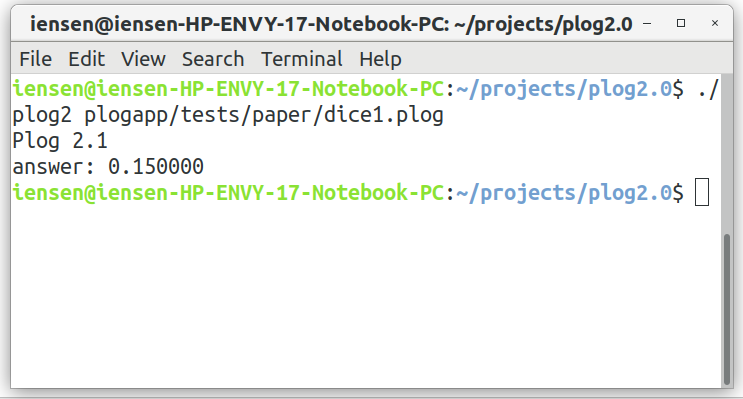
\includegraphics[width=0.9\textwidth]{plog_output.png}
\caption{P-log output}
\label{fig:plog_output}
\end{figure}

The solver also allows to compute possible worlds of a given program. For that, pass an option  \texttt{--mode=pw} to the solver.
For example, in order to compute possible worlds of a program stored in \texttt{plogapp/tests/causal/courtorder.plog}, run the command
\texttt{./plog2 --mode=pw  plogapp/tests/causal/courtorder.plog}, where plog2 is the system executable.
Below is an example output:
\begin{verbatim}
 ./plog2 --mode=pw plogapp/tests/causality/courtorder.plog 
Plog 2.1
Possible Worlds:
1: {court_order(0), court_order(1) = false, court_order(2) = false,
 court_order(3) = false, captain_order(1), captain_order(0) = false,
 captain_order(2) = false, captain_order(3) = false, 
shoot(a, 2), shoot(b, 2), shoot(a, 0) = false, 
shoot(a, 1) = false, shoot(a, 3) = false, shoot(b, 0) = false,
 shoot(b, 1) = false, shoot(b, 3) = false, dead(3), 
dead(0) = false, dead(1) = false, dead(2) = false}

Probabilities:
1: 1
\end{verbatim}
\st
The details of the syntax of the language can be found in \cite{Balai2019} and in the following sections. 

\section{Command Line Options}\label{option}

In this section we will describe the meanings of command line options supported by
P-log. As of right now, the system requires  a single argument which is a path to the p-log file.

\medskip\noindent
In addition, it supports the following named arguments:
\begin{itemize}
\item \texttt{--mode=X}, where \texttt{X} is one of \texttt{pw} or \texttt{query}. When \texttt{X} is \texttt{pw}, the solver computes possible worlds of a given program. Otherwise, it computes the probability of the query. The default value is \texttt{query}.
\end{itemize}

  \begin{itemize}
  \item \texttt{--algo=X}, where \texttt{X} is one of \texttt{naive} or \texttt{dco}. When \texttt{X} is \texttt{naive}, the solver uses naive algorithm to compute the query by computing possible worlds and iterating over all of them. The algorithm is similar to the translate algorithm from \cite{zhu2012plog}, but, unlike the implementation by its author, our uses a more modern ASP solver, Clingo. When \texttt{X} is \texttt{dco}, the solver uses special algorithm for dynamically causally ordered programs, described in \cite{balai2017investigating}, which can be more efficient. Note that when the input program is not dynamically causally ordered, and \texttt{X} is \texttt{dco}, the solver behavior is undefined. 
\end{itemize}
\st
See Section \ref{sysusage} for an example of using this argument.


\section{Syntax Description}


\subsection{Sort definitions}\label{ss}


This section starts with a keyword $sorts$ followed by a collection of sort definitions of the form: 

\begin{equation*}
  sort\_name=sort\_expression.
\end{equation*}
\textit{sort\_name} is an identifier preceeded by the pound sign (\#).
\textit{sort\_expression}  on the right hand side denotes a collection of strings called $a~sort$.



\st \textit{Basic sorts} are defined as named collections of numbers and \textit{identifiers}, i.e, strings consisting of

\begin{itemize}

 \item letters: $\{a,b,c,d,...,z,A,B,C,D,...,Z\}$

 \item digits: $\{0,1,2,...,9\}$

 \item underscore: $\_$

\end{itemize}

and starting with a lowercase letter.


\medskip\noindent
A \textit{non-basic sort} also contains at least one \textit{record} of the form $id(\alpha_1,\dots, \alpha_n)$ where $id$ is an identifier and 

$\alpha_1, \dots, \alpha_n$ are either identifiers, numbers or records. 



\st We define sorts by means of expressions (in what follows sometimes referred to as statements) of six types:
\begin{enumerate}


\item\label{numrange}
\textbf{numeric range} is of the form:
\begin{equation*}
number_1..number_2
\end{equation*}
where $number_1$ and $number_2$ are non-negative numbers such that $number_1 \le number_2$. The expression defines the set 

of sequential numbers \\$\{number_1, number_1+1, \dots, number_2\}$.



\textit{Example:}



\begin{verbatim}

 #sort1=1..3.

\end{verbatim}

\texttt{\#sort1} consists of numbers $\{1,2,3\}$.



\item\label{groundset} \textbf{set of ground terms} is of the form:

\begin{equation*}
\{t_1,..,,t_n\}
\end{equation*}
The expression denotes a set of \textit{ground terms} $\{t_1,...,t_n\}$, defined as follows:
\begin{itemize}
 \item numbers and identifiers are ground terms;
 \item If $f$ is an identifier and $\alpha_1, \dots, \alpha_n$ are ground terms, 
then $f(\alpha_1,\dots, \alpha_n)$ is a ground term.
\end{itemize}

\textit{Example}: 
\begin{verbatim}
 #sort1={f(a),a,b,2}.
\end{verbatim}
\item\label{recordset} \textbf{set of records} is of the form:

\begin{equation*}
f(sort\_name_1,..., sort\_name_n)
\end{equation*}
where $f$ is an identifier, for $ 1\leq i\leq n$, $sort\_name_i$ occurs in one of the preceeding sort definitions.

The expression defines a collection of ground terms 
\\ $\{f(t_1,\dots,t_n):  t_1 \in s_i \land \dots \land t_n \in s_n\}$

\textit{Example}
\begin{verbatim}
 #s1=1..2.
 #s2 = {a,b}.
 #sf=f(#s1, #s2)). 
\end{verbatim}

The sort \texttt{\#sf} consists of records $\{f(1,1,2),f(1,1,1),f(2,1,1)\}$



 \item\label{setexpr} \textbf{set-theoretic expression} is in one of the following forms:
\begin{itemize}
\item $\#sort\_name$  
\item an expression of the form 1, 2, or 3, denoting a set of ground terms
\item $(S_1 \bigtriangledown S_2)$, where $\bigtriangledown \in \{+,-,*\}$ and both $S_1$ and $S_2$ are set theoretic expressions
\end{itemize}

$\#sort\_name$ must be a name of a sort occurring in one of the preceeding sort definitions. 
The operations $+$ $*$ and $-$ stand for union, intersection and difference correspondingly.


\textit{Example} : 
\begin{verbatim}
 #sort1={a,b,2}.
 #sort2={1,2,3} + {a,b,f(c)} + f(#sort1).
\end{verbatim}
 \texttt{\#sort2} consists of ground terms $\{1,2,3,a,b,f(c),f(a),f(b),f(2)\}$.

\end{enumerate}

\subsection{Attribute Declarations}

\noindent  The second part of a  P-log program starts with the keyword \texttt{attributes}
and is followed by statements of the form

\begin{equation*}
attr\_symbol : \#sortName_1,\dots,\#sortName_n \rightarrow \#sortName  
\end{equation*}
where $attr\_symbol$ is an identifier (in what follows referred to as an attribute symbol) and
$\#sortName$, $\#sortName_1$,\dots,$\#sortName_n$ are sorts defined in sort definitions section of the program.



Multiple declarations containing the same attribute symbol are not allowed.
Attributes with no arguments must be declared as $attr\_symbol:sortName_1$ (example: \texttt{a:\#bool}).

% \st For any sort name $\#s$, the system includes declaration  $\#s:\#s -> #boolean$ automatically. 

\subsection{Program Statements}

\st The third part of a P-log program starts with the keyword \textit{statements} followed by a collection \textit{rules} and \textit{pr-atoms} (in any order). Here we give a brief overview of the system assuming that a reader is familiar with notions of a term and a literal. For the details, please refer to \cite{Balai2019}. 

\subsubsection{Program Rules}
P-log rules are of the following form:

\begin{equation}
   a(t) = y \leftarrow l_1,  \ldots, l_k, not~l_{k+1} \ldots not~l_{n}.
 \end{equation}
where $a(t) = y$ is a program atom and $l_1,\ldots,l_k$ are program literals.
The atom $a(t) = y$ is referred to as the \textit{head} of the rule, and $l_1,\ldots,l_k$ is referred to as the \textit{body} of the rule.
 A rule with $k=0$ is referred to as a \textit{fact}.
 The system allows for a shorthand $a(t)$ for $a(t) = true$, and standard arithmetic relations of the form $t_1~op~t_2$, where $op \in \{\texttt{>=},\texttt{<=},\texttt{>},\texttt{<},\texttt{=},\texttt{!=}\}$ in the body of the rule .
 Three special kinds of rules are \textit{random selection rules}, \textit{observations} and \textit{actions}.
 As defined in \cite{Balai2019},
 random selection rule is a rule whose head is of one of the forms $random(a,p)$ or $random(a)$. Action is a fact whose head is $do(a,y)$\footnote{The system doesn't support rule labels and actions of the form $do(r,a,y)$ defined in \cite{Balai2019}. Therefore there has to be at most one action of each attribute term. This is a limitation we plan to overcome in future.}.
 Observation is a fact whose head is of the form $obs(a,y)$ \textcolor{red}{Right now, the system only supports observations and actions whose arguments are positive atoms}.

 \subsubsection{Pr-Atoms}

 Probability atoms (in short, pr-atoms) are of the form 
 $$pr(a(t) = y | B) = v.$$
 where $a(t) = y$ is a program atom, $B$ is a collection of e-literals and $v$  written as a fraction of the form $n/m$, where $n$ and $m$ are natural numbers.  Example:
\begin{center}
 \texttt{pr(roll(D)=6 | not owns(D,mike))=1/4.}
\end{center}
 \subsection{Program Examples}

 For a collection of working P-log programs used for system testing and development, please refer to
 \begin{center}
\url{https://github.com/iensen/plog2.0/tree/master/plogapp/tests}.
 \end{center}
 

 \section{Error Checking}

 \textcolor{red}{Please be aware that some of the errors are not implemented yet.}

\st
In this section, we describe  additional errors which are detected when no syntax error is found.
The majority of the errors are related to types.
\subsection{Type errors}
Type errors are considered as serious issues which make it  impossible to compile and execute the program.
Type errors can occur in all four sections of a P-log program.
\subsubsection{Sort definition errors}
The following are possible causes of a sort definition error  that will result in a type error  message.
\begin{enumerate}
\item A numeric range $n_1..n_2$ (statement \ref{numrange} in section \ref{ss}) where  $n_1$ is greater than $n_2$.

\textit{Example:}
\begin{verbatim}
 sorts
 #s=100500..1.
\end{verbatim}


\item  A set-theoretic expression (statement \ref{setexpr} in section \ref{ss}) containing a sort name that has not been defined.

\textit{Example:}
\begin{verbatim}
 sorts
 #s={a}.
 #s2=#s1-#s.
\end{verbatim}

\item  Declaring a sort more than once.

\textit{Example:}
\begin{verbatim}
 sorts
 #s={a}.
 #s={b}.
\end{verbatim}

\item A record definition (statement \ref{recordset} in section \ref{ss}) that contains an undefined sort.

\textit{Example:}
\begin{verbatim}
 sorts
 #s=1..2.
 #fs=f(s,s2).
\end{verbatim}
\end{enumerate}
\subsubsection{Attribute declarations errors}

\begin{enumerate}
\item An attribute with the same name is declared more than once.
\textit{Example:}
\begin{verbatim}
 sorts
 #s={a}.
 attributes
 a: #s -> #s.
 a: #s,#s ->#s.
\end{verbatim}
\item An attribute declaration contains an undefined sort.
\textit{Example:}
\begin{verbatim}
 sorts
 #s={a}.
 attributes
 p:#ss.
\end{verbatim}

\item An attribute name coincides with the name of a record belonging to one of the sorts.
\textit{Example:}
\begin{verbatim}
 sorts
 #s1={f(a)}.
 #s2 = {1,2,3}.
 attributes
 f:#s1.
\end{verbatim}
Here there is an attribute named $f$ and a record $f(a)$ belonging to \texttt{\#s1}.
\end{enumerate}
\subsubsection{Errors in program statements}

To describe errors in program statement, we need an auxiliary definition of a term.
\begin{enumerate}
 \item numbers, identifiers and variables are \textit{terms};
 \item If $f$ is an identifier and $\alpha_1, \dots, \alpha_n$ are \textit{terms}, 
   then $f(\alpha_1,\dots, \alpha_n)$ is a \textit{term}.
 \item\label{arithterms} standard arithmetic expressions constructed from numbers, variables and operators $+$, $-$ , $*$, $/$ are terms. 
\end{enumerate}

\medskip\noindent
We will refer to terms of the form \ref{arithterms} as \textit{arithmetic terms}.

\medskip\noindent
For each literal $\tau_1 \odot \tau_2$ occurring in a program,  $\odot \in \{>, \leq, \geq, =, \not=, <\}$, where $\tau_1$, $\tau_2$ are terms, we will produce errors in the following cases:

\begin{enumerate}
  
\item $\tau_2$ is of the form $f(t_1,\ldots,t_n)$, $f$ is an attribute name;
\item $\tau_1$ is of the form $f(t_1,\ldots,t_n)$, $f$ is an attribute name, and $\odot \not\in\{=,\not=\}$;
\item $\tau_1$ is of the form $f(t_1,\ldots,t_n)$, $f$ is an attribute declared as:
  $$f: s_1,\ldots,s_m \rightarrow s_{m+1}$$
  where $n \not=m$
  
\item $\tau_1$ is of the form $f(t_1,\ldots,t_n)$, $f$ is an attribute declared as:
  $$f: s_1,\ldots,s_n \rightarrow s_{n+1}$$
  and for some $i \in 1...n$, $t_i$ is a ground term not belonging to $s_i$;
  
\item $\tau_1$ is of the form $f(t_1,\ldots,t_n)$, $f$ is an attribute declared as:
  $$f: s_1,\ldots,s_n \rightarrow s_{n+1}$$
  and $\tau_2$ is a ground term such that $\tau_2 \not\in s_{n+1}$.
  
\end{enumerate}


\subsection{Type warnings}\label{type_warnings}

\textcolor{red}{This section is to be completed and implemented. At the very least, we plan to support
  finite-domain constraint-based typechecking which will flag rules with no ground instances. In addition, we fill flag empty sorts. There should be a user option to disable both warnings.}

\bibliography{mybib}
\bibliographystyle{plain}
\end{document}


%%% Local Variables:
%%% mode: latex
%%% TeX-master: t
%%% End:
